\documentclass{beamer}
%\documentclass[handout]{beamer}

\usepackage{ensislides}
\usepackage[utf8]{inputenc}
\usepackage[OT1]{fontenc}
\usepackage[french]{babel}

\setbeamertemplate{caption}[default]


\title[Visu Scientifique]{Visualisation Scientifique}

\subtitle{Soutenance} % (optional)

\author{Yoan Souty\\Antonin Klopp-Tosser}
% - Use the \inst{?} command only if the authors have different
%   affiliation.

\institute{Ensimag}

\date{Lundi 3 Décembre}

\begin{document}

\begin{frame}
  \titlepage
\end{frame}

\section[Intro]{Introduction}


\begin{frame} \frametitle{Fonctionnalités}

  \begin{block}{Lancement du script}
    \begin{itemize}
      \item \texttt{./main.sh <type> [--help|--default|--iso|--temp]}
      \item \texttt{type} : SP1, SP2
      \item \texttt{--help} : affichage de l'aide
      \item \texttt{--iso} : animation avec courbes iso-valeurs
      \item \texttt{--temp} : animation avec températures
      \item \texttt{--default} : (ou sans argument), animation températures + iso-valeurs + lignes de courant
    \end{itemize}
  \end{block}

  Relance automatique des requêtes en cas d'échec au bout de 30 secondes
\end{frame}


\section[Températures]{Carte des températures}


\begin{frame} \frametitle{Génération des cartes de températures}
  \begin{itemize}
    \item Échelle de températures indexée sur celle de Météo France
  \end{itemize}

  \begin{figure}
    \centering
    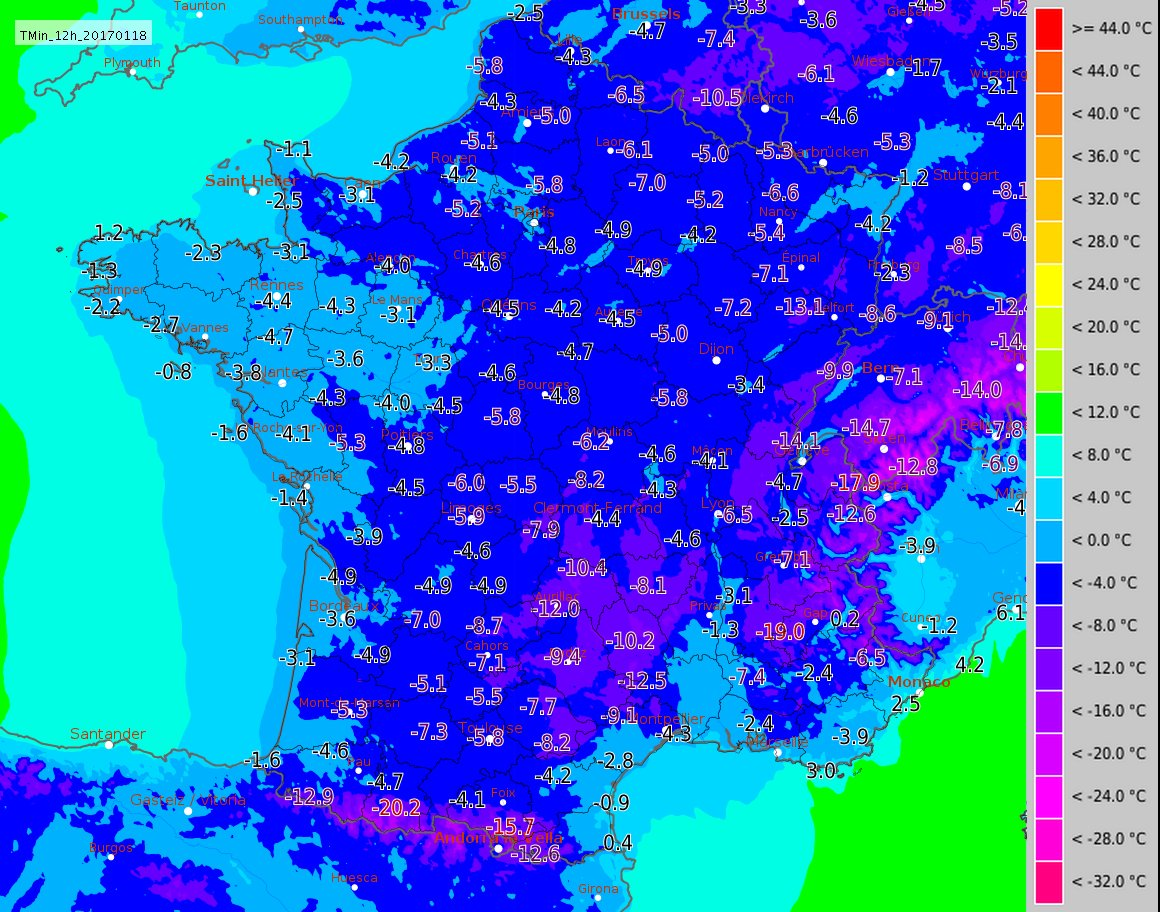
\includegraphics[width=\textwidth,height=0.8\textheight,keepaspectratio]{fig/meteo_fr_scales_temp}
  \end{figure}

\end{frame}

\begin{frame} \frametitle{Exemple}
  \begin{figure}
    \centering
    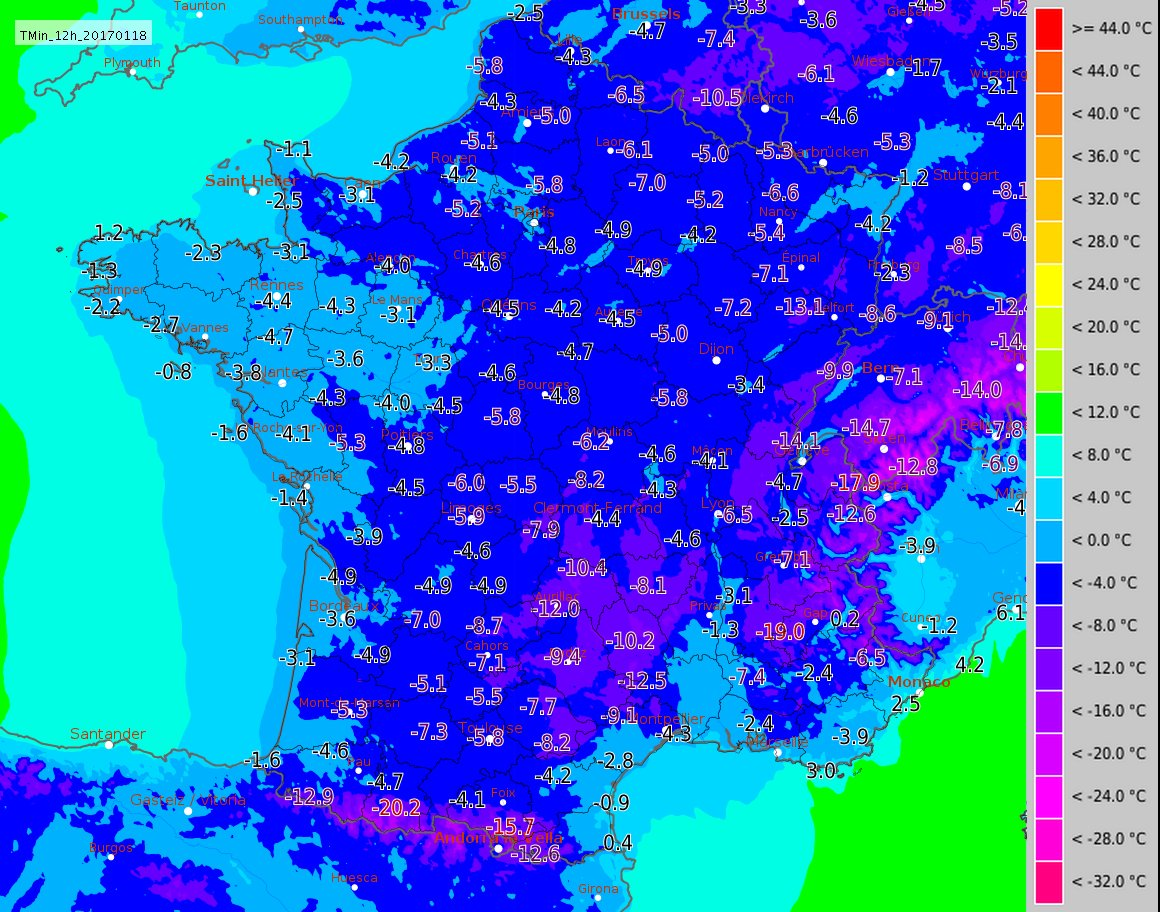
\includegraphics[width=\textwidth,height=0.8\textheight,keepaspectratio]{fig/meteo_fr_scales_temp}
  \end{figure}
  \pause
  \begin{figure}
    \centering
    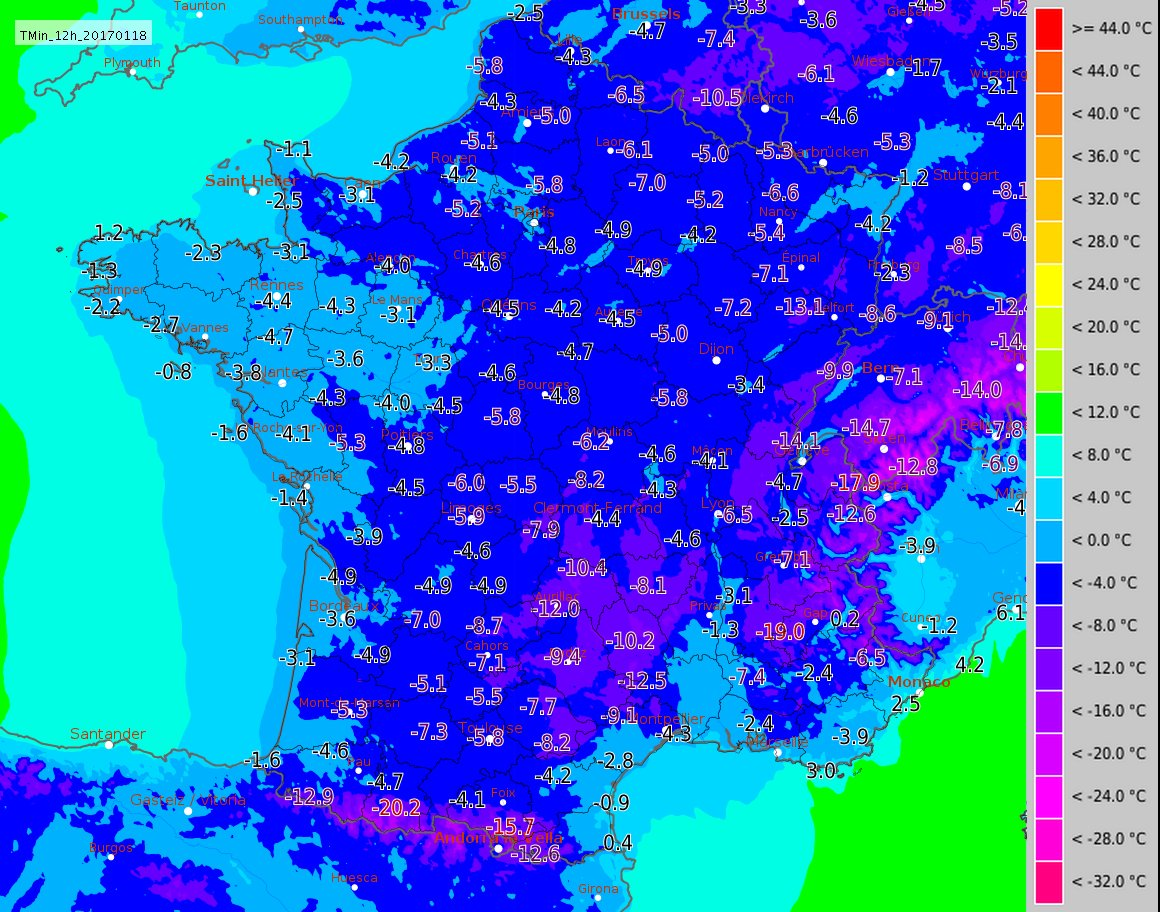
\includegraphics[width=\textwidth,height=0.8\textheight,keepaspectratio]{fig/meteo_fr_scales_temp}
  \end{figure}

  \pause
  \begin{figure}
    \centering
    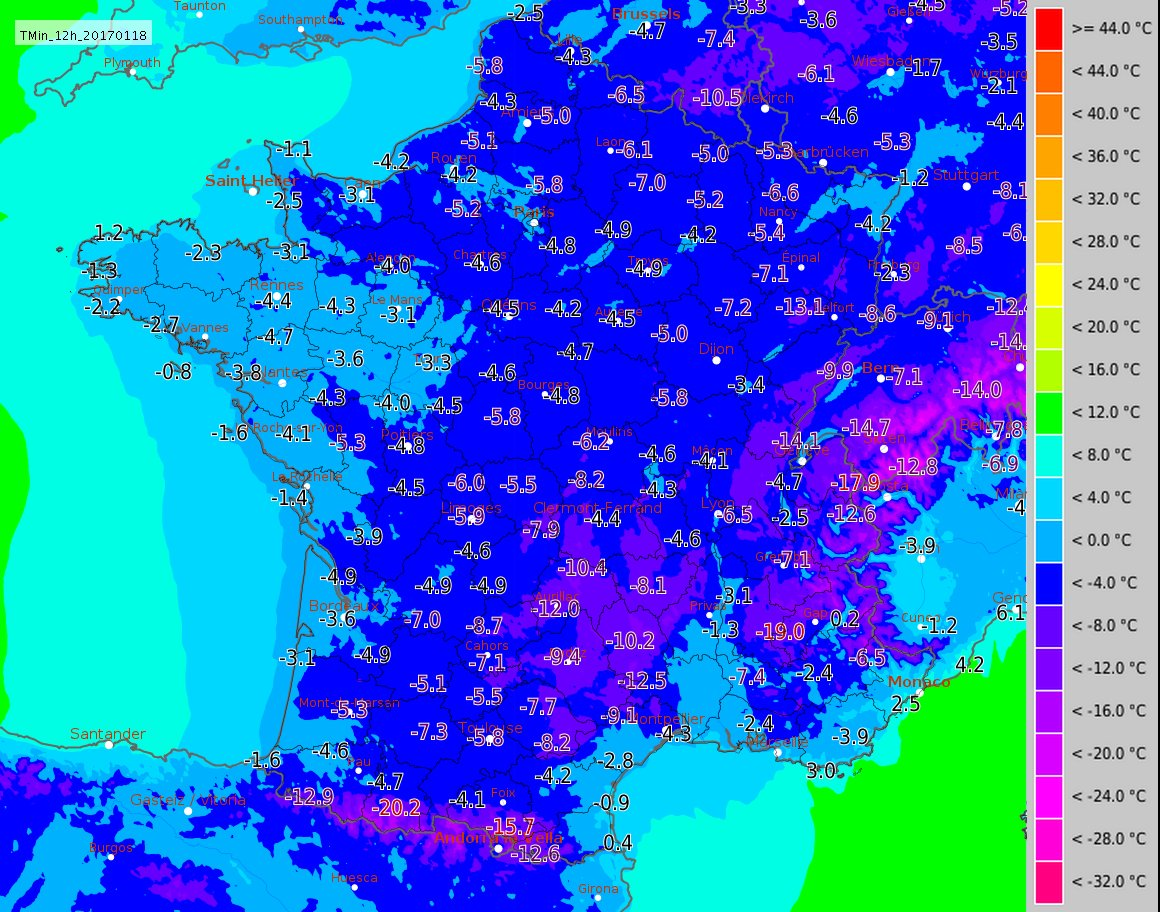
\includegraphics[width=\textwidth,height=0.8\textheight,keepaspectratio]{fig/meteo_fr_scales_temp}
  \end{figure}

  \pause
  \begin{figure}
    \centering
    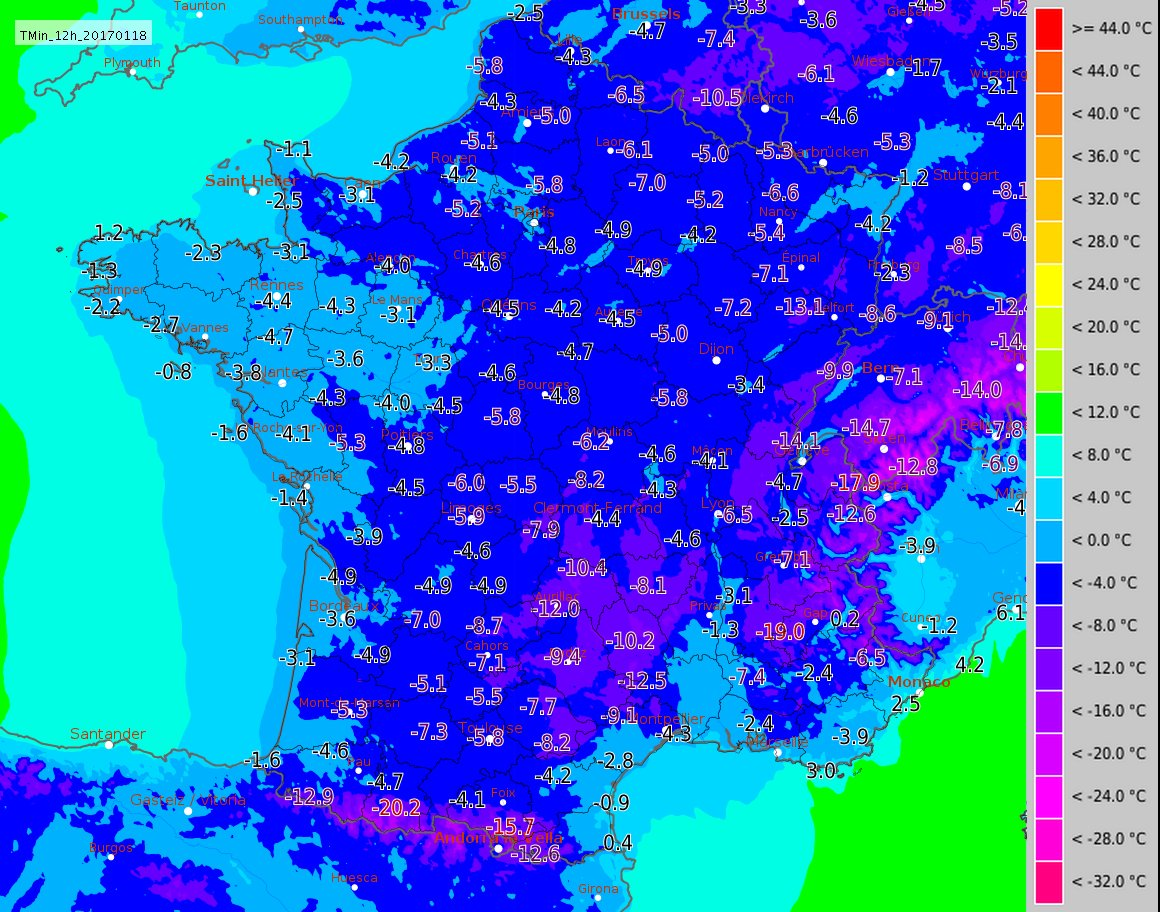
\includegraphics[width=\textwidth,height=0.8\textheight,keepaspectratio]{fig/meteo_fr_scales_temp}
  \end{figure}
\end{frame}


\section[Isovaleurs]{Lignes iso-valeurs}

\begin{frame}
  \frametitle{Génération des lignes iso-valeurs}
  \begin{block}{Titre d'un bloc}
    \begin{itemize}
      \item Un point d'un bloc
    \end{itemize}
    Texte standard
  \end{block}

  \begin{alertblock}{Bloc d'alerte}
    Oulala il faut faire attention
  \end{alertblock}

  \begin{exampleblock}{Bloc d'exemple}
    Par exemple, on a ..
  \end{exampleblock}
\end{frame}

\section[Lignes de courant]{Lignes de courant}

\begin{frame}
  \frametitle{Génération des lignes de courant}
  \begin{columns}[T,totalwidth=\textwidth] % option T for best results ?
  \begin{column}{5cm}
  \begin{block}{Colonne 1}
    Texte dans la\\
    colonne 1.
  \end{block}
  \end{column}

  \begin{column}{5cm}
  \begin{block}{Colonne 2}
    Texte dans la
    colonne 2 qui peut être
    plus long que dans la
    colonne 1.
  \end{block}
  \end{column}
 \end{columns}
\end{frame}

\begin{frame}
  \frametitle{Exemple}
  \begin{columns}[T,totalwidth=\textwidth] % option T for best results ?
  \begin{column}{5cm}
  \begin{block}{Colonne 1}
    Texte dans la\\
    colonne 1.
  \end{block}
  \end{column}

  \begin{column}{5cm}
  \begin{block}{Colonne 2}
    Texte dans la
    colonne 2 qui peut être
    plus long que dans la
    colonne 1.
  \end{block}
  \end{column}
 \end{columns}
\end{frame}


\section{Visualisation complète}


\end{document}


%%% Local Variables:
%%% mode: latex
%%% TeX-master: t
%%% End:
